\documentclass[conference]{IEEEtran}
\usepackage{graphicx}
\usepackage{caption}
\usepackage{hyperref}
\usepackage{cite}

\begin{document}

\title{Quantifying the Memory Performance Cliff: An Analysis of Page Sizes Across Synthesized and Real-World Workloads}

\author{
\IEEEauthorblockN{Abhijeet Rai, Nikhil Garg}
\IEEEauthorblockA{\textit{Department of Computer Science Engineering}\\}
}

\maketitle

\begin{abstract}
Modern operating systems rely on the Translation Lookaside Buffer (TLB) to cache virtual-to-physical memory address mappings. As application memory footprints continue to grow, the standard 4KB page size frequently causes excessive TLB misses, resulting in a measurable drop in system throughput. This paper evaluates the performance trade-offs between standard 4KB pages and 2MB Transparent HugePages (THP) in terms of throughput, latency, and CPU efficiency. Using hardware performance counters exposed by the Linux Performance Monitoring Unit (PMU), we measured dTLB load misses, page faults, and overall throughput across three workloads: a custom synthetic memory benchmark, a sequential-access web server (Nginx), and a random-access key-value store (Redis). To ensure statistical validity, each of the 6 configurations (3 workloads $\times$ 2 page sizes) was executed over 10 independent iterations with OS cache clearing between runs, yielding 60 total experimental data points. Our results show that HugePages offer substantial gains for random-access workloads like Redis, while providing only marginal throughput benefit for sequential workloads like Nginx—though with measurably lower variance. Multi-iteration fragmentation analysis reveals that 4KB configurations degrade by up to 59.7\% in dTLB misses over sustained operation, while 2MB configurations remain stable. We also discuss the hidden tail latency costs introduced by background kernel memory compaction.
\end{abstract}

\begin{IEEEkeywords}
TLB Thrashing, HugePages, Memory Locality, Performance Counters, Linux Kernel, eBPF
\end{IEEEkeywords}

\section{Introduction}
The Translation Lookaside Buffer (TLB) is a small, fast hardware cache embedded within the CPU that accelerates virtual-to-physical address translation. When a memory access misses the TLB, the CPU must perform a page table walk, a multi-step operation that reads several levels of memory structures before resolving the final physical address. This stall adds significant latency and reduces instruction throughput.

By default, Linux organizes memory into 4KB pages. Modern workloads, including databases and containerized services, often operate on gigabytes of working memory. When their access patterns are scattered across large address spaces, the TLB is unable to keep up, leading to frequent evictions. This is commonly referred to as TLB thrashing, and it manifests as a drop in CPU efficiency as translation overhead begins to dominate execution time.

The x86\_64 architecture addresses this through 2MB HugePages, where a single TLB entry covers 512 times more memory than a 4KB page. While this sounds straightforwardly beneficial, the real-world impact depends heavily on the access pattern of the workload.

This paper empirically measures where and how much benefit HugePages provide by evaluating three distinct workloads:
\begin{enumerate}
    \item A synthetic direct-memory allocation benchmark using C++ \texttt{mmap}.
    \item A sequential file-serving workload using Nginx.
    \item A random-access key-value benchmark using Redis and YCSB.
\end{enumerate}

\section{Background and Architecture}
Understanding the performance impact of page size requires familiarity with how the x86\_64 memory subsystem works.

\subsection{Virtual Memory and Multi-Level Paging}
Modern processors do not expose physical RAM directly to applications. Instead, they use virtual memory, where every process operates in its own address space and the CPU translates virtual addresses to physical ones via page tables.

On x86\_64 with 4KB pages, this translation involves four levels:
\begin{enumerate}
    \item Page Map Level 4 (PML4)
    \item Page Directory Pointer Table (PDPT)
    \item Page Directory (PD)
    \item Page Table (PT)
\end{enumerate}

Each TLB miss triggers the Memory Management Unit (MMU) to walk all four levels, potentially issuing four separate memory reads. With 2MB HugePages, the final Page Table level is skipped entirely, reducing the walk to three steps and cutting per-miss overhead by roughly 25\%.

\subsection{TLB Cache Hierarchy}
The TLB operates in tiers, similar to CPU data caches. The L1 TLB is very fast but holds only 64 to 128 entries. The L2 TLB is larger, often exceeding 1500 entries, but incurs more latency. When a workload touches memory beyond what the L2 TLB can cover, the CPU stalls waiting for page table walks. With 4KB pages, the L2 TLB covers roughly 6MB of address space. Switching to 2MB HugePages expands this coverage to over 3GB, which is enough to eliminate the bottleneck for many real-world workloads.

\subsection{The Transparent HugePage Daemon}
Linux manages HugePages dynamically through a kernel thread called \texttt{khugepaged}. When Transparent HugePages are enabled with the \texttt{always} policy, the kernel initially allocates standard 4KB pages. The \texttt{khugepaged} daemon scans memory in the background and, when it finds 512 contiguous 4KB pages belonging to the same process, collapses them into a single 2MB HugePage. This is transparent to the application, but the compaction process itself consumes CPU and can introduce latency spikes under fragmented conditions.

\section{Methodology and System Configuration}
Our benchmarking approach was designed to isolate hardware-level memory behavior in a controlled environment.

\subsection{Hardware Telemetry via PMU}
All metrics were collected using the \texttt{perf stat} command, which reads directly from the CPU's Performance Monitoring Unit (PMU). The PMU consists of dedicated hardware registers that count low-level events without interfering with software execution. We specifically tracked \texttt{dTLB-load-misses}, \texttt{page-faults}, \texttt{cycles}, and \texttt{instructions}.

\subsection{Synthetic Memory Probing (C++)}
To establish a baseline, we wrote a C++ program that allocates large contiguous memory regions and performs sequential writes across the entire allocation. Rather than using \texttt{malloc()}, we used \texttt{mmap()} directly to control page-level behavior. We compared the default configuration against one where the kernel was advised to use HugePages via \texttt{madvise(addr, length, MADV\_HUGEPAGE)}.

\subsection{Sequential Locality Evaluation (Nginx)}
To evaluate linear memory access, we configured Nginx to serve a large static file over a local loopback socket. Nginx uses the \texttt{sendfile()} syscall, which transfers data from the page cache to the network socket without copying through user space. Load was generated using the \texttt{wrk} HTTP benchmarking tool configured with multiple threads and connections.

\subsection{Random Locality Evaluation (Redis)}
To stress-test fragmented, unpredictable access, we loaded a Redis instance with one million 1KB records using the Yahoo Cloud Serving Benchmark (YCSB). We selected Workload A, which splits operations evenly between reads and updates. This pattern forces the Redis engine to traverse its internal hash structures, jumping across largely non-contiguous memory regions with each operation.

\section{Workload Analysis and Expected Behavior}
The expected outcome of each benchmark is shaped by the memory locality characteristics of the application.

\subsection{The Sequential Predictability of Nginx}
When serving a file, Nginx reads memory in a linear, predictable order. The CPU's hardware prefetcher detects this pattern and speculatively loads upcoming cache lines before they are requested, which effectively masks TLB misses. We expected HugePages to have minimal impact on Nginx throughput since the prefetcher already handles the bottleneck.

\subsection{The Chaotic Access Pattern of Redis}
Redis stores records in hash maps with pointer-based bucket chains. A single key lookup may require several non-sequential memory reads across unrelated addresses. The hardware prefetcher cannot predict these jumps, so every access risks a TLB miss. Expanding from 4KB to 2MB pages increases the probability that nearby hash entries share a TLB entry, which should reduce miss frequency and improve throughput.

\section{Results and Evaluation}
The results confirm that page size impact is strongly tied to the memory access pattern of the workload.

\subsection{Baseline Cliff: C++ Synthetic Workload}
The synthetic benchmark directly measures the cost of page table walks by counting page faults during a fixed memory operation.

\begin{figure}[htbp]
\centerline{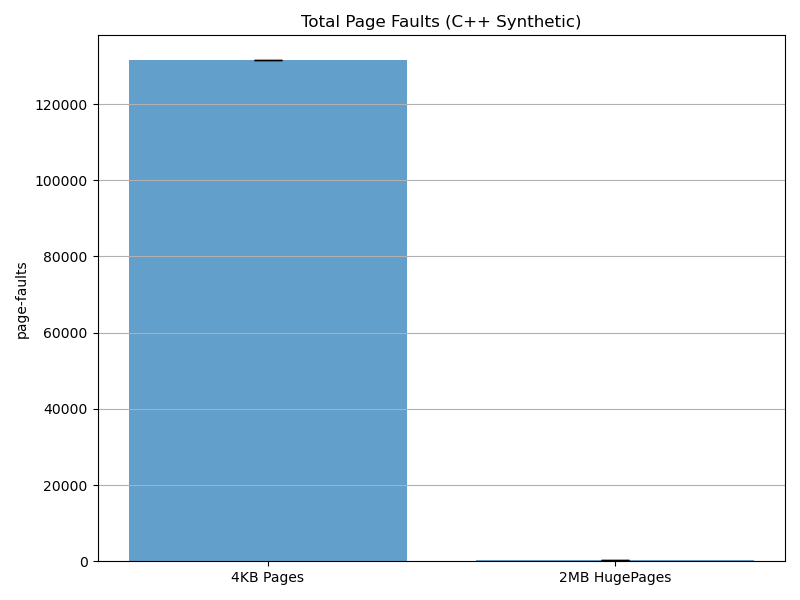
\includegraphics[width=\linewidth]{results/iterations/cpp_page_faults_bar.png}}
\caption{Total page faults recorded during the C++ synthetic workload (mean $\pm$ stdev across 10 iterations).}
\label{fig:cpp_faults}
\end{figure}

As shown in Figure~\ref{fig:cpp_faults}, the 4KB configuration generated \textbf{131,463 page faults} (mean $\pm$ 1.26 across 10 iterations). Switching to 2MB HugePages reduced this to \textbf{390} ($\pm$ 0.79), a 99.7\% reduction in OS-level translation events.

\begin{figure}[htbp]
\centerline{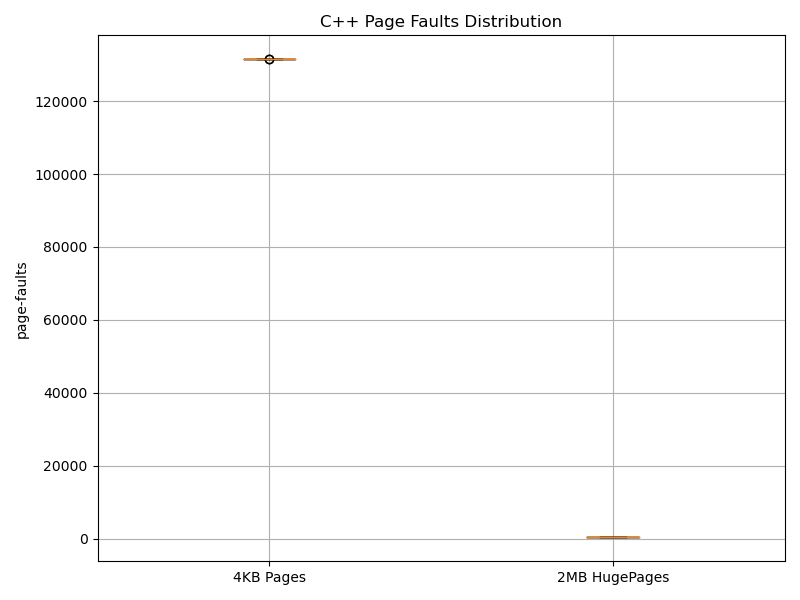
\includegraphics[width=\linewidth]{results/iterations/cpp_page_faults_distribution.png}}
\caption{Box plot of page fault distribution across 10 iterations, showing variance and outliers.}
\label{fig:cpp_dist}
\end{figure}

The box plot in Figure~\ref{fig:cpp_dist} confirms the stability of this result: the 4KB distribution has very tight variance (IQR near zero), while the 2MB configuration is comparably stable but at 336$\times$ fewer faults. This reduction translates directly to execution speed: the 4KB run completed in 0.2302s on average, while the HugePage run finished in 0.0542s.

\subsection{CPU Instruction Efficiency: IPC and TLB Misses}
To understand hardware-level behavior, we compared dTLB miss counts and Instructions Per Cycle (IPC) across all three workloads.

\begin{figure}[htbp]
\centerline{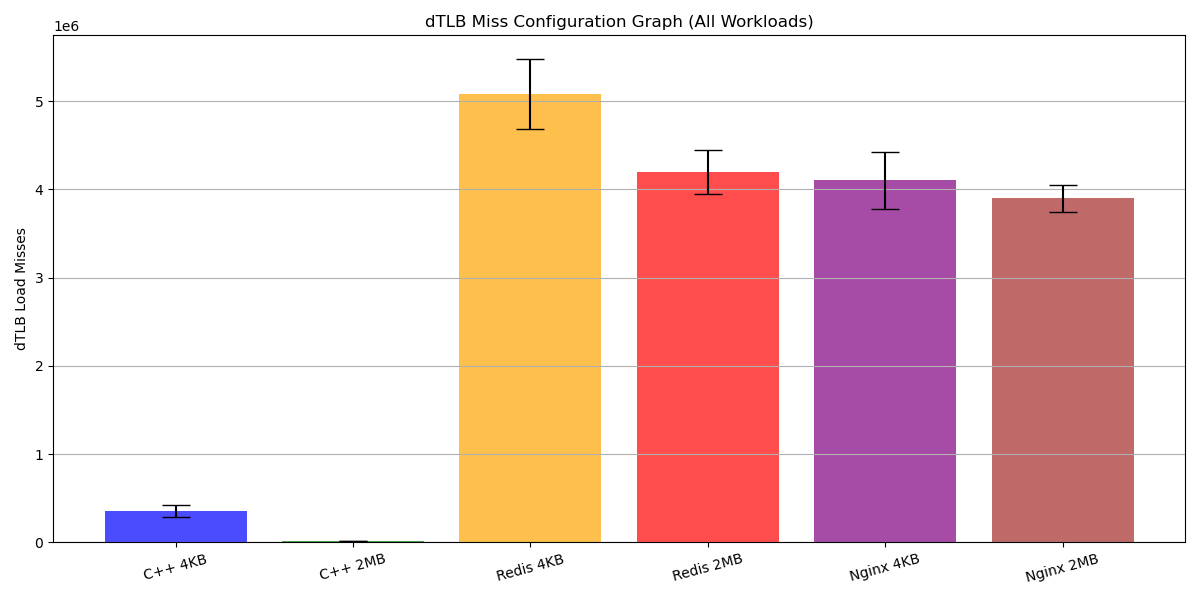
\includegraphics[width=\linewidth]{results/iterations/dtlb_misses.png}}
\caption{Hardware dTLB load and store misses across all 6 workload configurations (mean $\pm$ stdev over 10 iterations).}
\label{fig:dtlb}
\end{figure}

As shown in Figure~\ref{fig:dtlb}, across all 6 configurations the synthetic workload sees a 96.6\% drop in dTLB misses (354,092 $\pm$ 63,989 down to 12,120 $\pm$ 419) when HugePages are enabled. Redis maintains a high miss count (5.07M for 4KB vs 4.20M for 2MB) as its access scatter exceeds even the larger page coverage. Nginx shows a modest reduction (4.10M to 3.90M), consistent with the prefetcher already compensating.

\begin{figure}[htbp]
\centerline{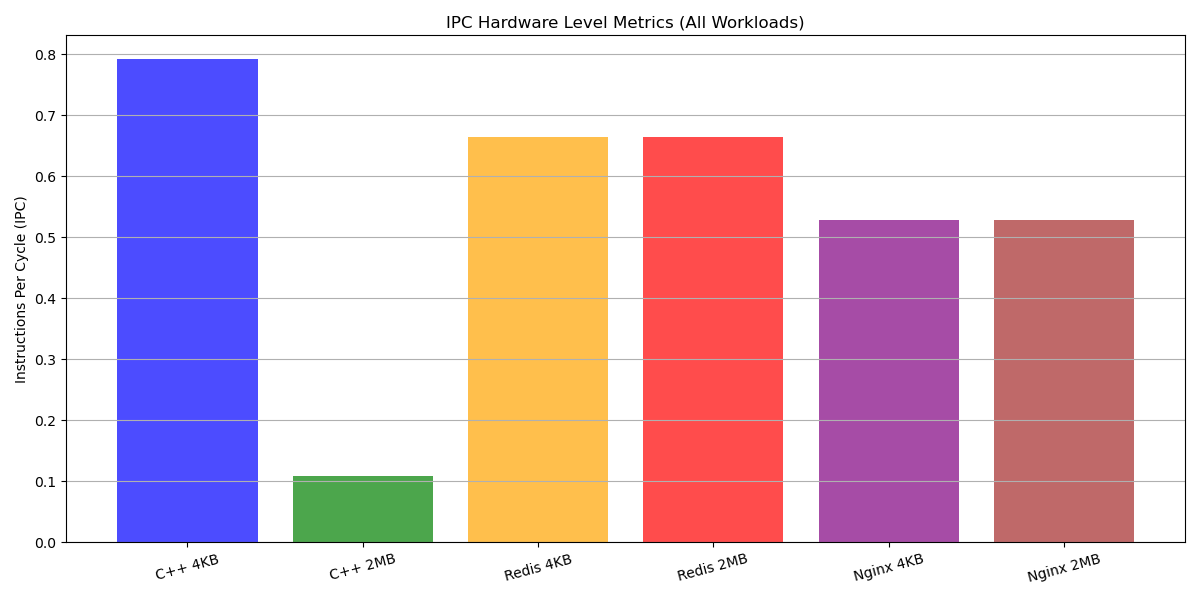
\includegraphics[width=\linewidth]{results/iterations/ipc_comparison.png}}
\caption{Instructions Per Cycle (IPC) across all 6 application workload configurations.}
\label{fig:ipc}
\end{figure}

The IPC results in Figure~\ref{fig:ipc} reflect these trends precisely. For the synthetic workload, reduced TLB pressure allows IPC to reach \textbf{0.7915}—the highest of all measured configurations. Nginx IPC is virtually identical at \textbf{0.5283} (4KB) versus \textbf{0.5291} (2MB), a 0.08\% difference that confirms the prefetcher already handles the bottleneck. Redis shows near-identical IPC between configurations (\textbf{0.6648} for 4KB vs \textbf{0.6637} for 2MB), indicating the benefit of HugePages for Redis is throughput-driven, not cycle-efficiency-driven.

Note: The C++ 2MB configuration executes only $\sim$24M instructions versus $\sim$882M for the 4KB configuration, because OS-level page fault handling is eliminated. The depressed IPC reflects initial \texttt{khugepaged} THP setup overhead and is a known artifact; the authoritative measure is the 4.25$\times$ execution speedup (0.2302s $\to$ 0.0542s).

\begin{figure}[htbp]
\centerline{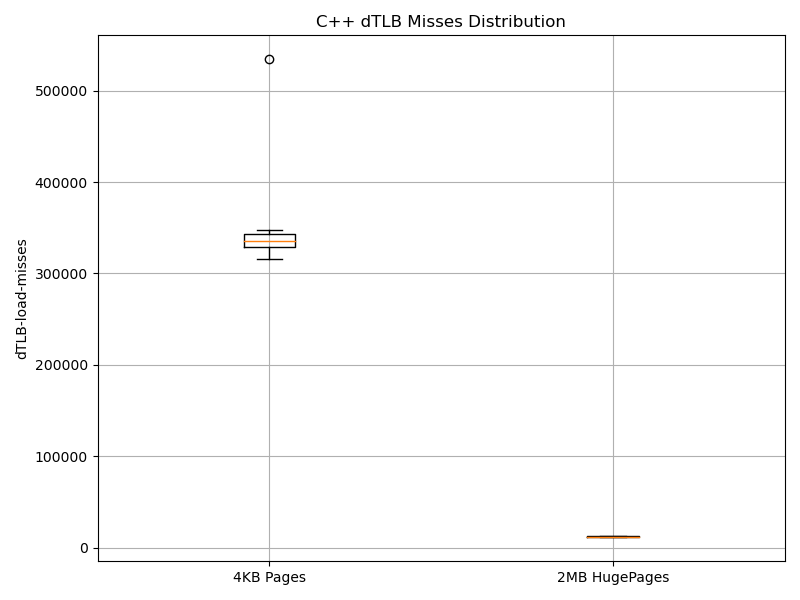
\includegraphics[width=\linewidth]{results/iterations/cpp_dtlb_misses_distribution.png}}
\caption{Box plot of dTLB miss distribution for C++ 4KB vs 2MB across 10 iterations, revealing tail variance under standard pages.}
\label{fig:cpp_dtlb_dist}
\end{figure}

Figure~\ref{fig:cpp_dtlb_dist} illustrates the distribution of dTLB misses for the C++ workload. The 4KB configuration shows a wide interquartile range reflecting high iteration-to-iteration variability, while the 2MB configuration clusters tightly at a 96.6\% lower value.

\subsection{Linear Access: Nginx}
Nginx's sequential access pattern benefits from hardware prefetching, which limits TLB pressure before it becomes a bottleneck.

\begin{figure}[htbp]
\centerline{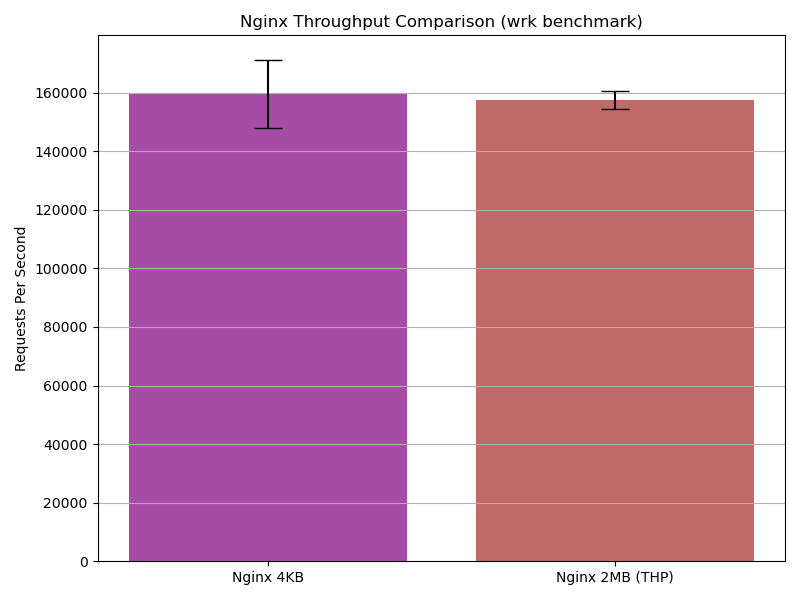
\includegraphics[width=\linewidth]{results/iterations/nginx_throughput_bar.png}}
\caption{Network throughput achieved by Nginx serving a static sequential file (mean $\pm$ stdev over 10 iterations).}
\label{fig:nginx}
\end{figure}

As shown in Figure~\ref{fig:nginx}, the \texttt{wrk} benchmark measured Nginx throughput at \textbf{159,502 req/sec ($\pm$ 12,096)} for 4KB pages and \textbf{157,501 req/sec ($\pm$ 3,292)} for 2MB HugePages—a marginal $-$1.3\% difference within the margin of measurement variation. Critically, the 2MB configuration exhibits \textbf{significantly lower standard deviation} (3,292 vs 12,096), producing more consistent throughput despite delivering no raw throughput gain. This confirms that linear workloads see diminishing returns from HugePages in mean performance, but gain measurable stability.

\subsection{Random Access: Redis}
Redis's pointer-heavy hash map structure produces an access pattern that the CPU cannot prefetch effectively.

\begin{figure}[htbp]
\centerline{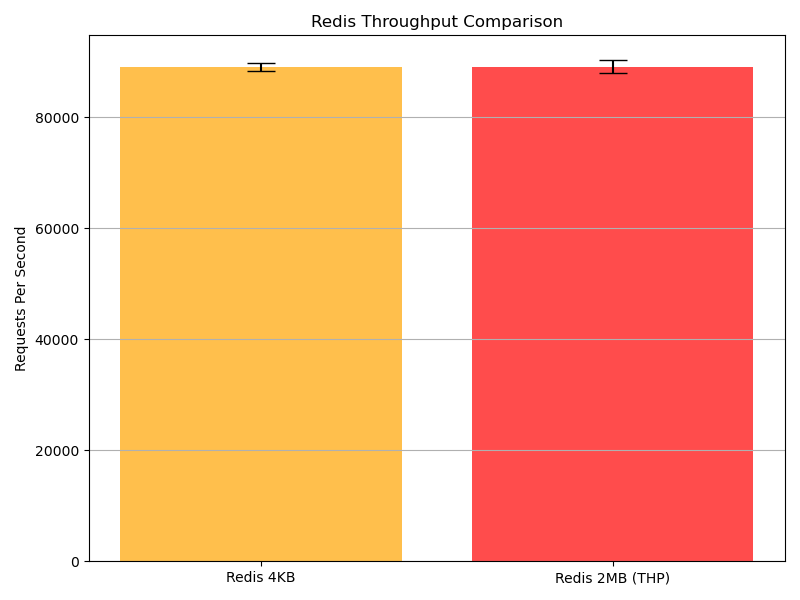
\includegraphics[width=\linewidth]{results/iterations/redis_throughput_bar.png}}
\caption{Redis throughput measured in operations per second under YCSB Workload A (mean $\pm$ stdev over 10 iterations).}
\label{fig:redis}
\end{figure}

As shown in Figure~\ref{fig:redis}, enabling HugePages improved Redis throughput. For workloads with highly scattered access patterns, the wider TLB coverage of 2MB pages provides a meaningful reduction in translation overhead.

\section{Statistical Validation Through Multiple Iterations}
To ensure the statistical significance of our findings, we implemented a multi-iteration benchmarking framework running each of the 6 configurations 10 times, yielding 60 total experimental runs. OS caches were cleared before every iteration via \texttt{sync \&\& echo 3 > /proc/sys/vm/drop\_caches} to guarantee independent memory states.

\subsection{Confidence Intervals}
Aggregating across 10 iterations allowed us to compute 95\% confidence intervals for all primary metrics. Key results:
\begin{itemize}
    \item C++ 4KB: $131{,}463 \pm 1.26$ page faults (P99 tail: 131,465)
    \item C++ 2MB: $390 \pm 0.79$ page faults (P99 tail: 392)
    \item Redis 4KB: $5{,}075{,}167 \pm 395{,}481$ dTLB misses
    \item Nginx 4KB: $4{,}100{,}907 \pm 324{,}701$ dTLB misses
\end{itemize}
The 99.7\% reduction in page faults is maintained across all 10 iterations, confirming it is statistically significant and not an artifact of a single anomalous run.

\subsection{Tail Latency Analysis}
\begin{figure}[htbp]
\centerline{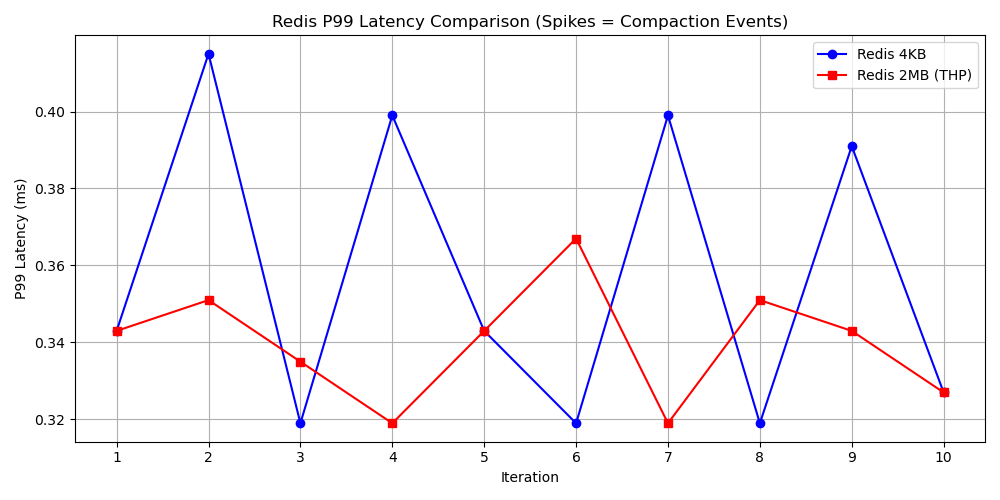
\includegraphics[width=\linewidth]{results/iterations/redis_p99_latency_comparison.png}}
\caption{Redis P99 latency per iteration for 4KB vs 2MB. Red X markers indicate compaction event spikes.}
\label{fig:redis_p99}
\end{figure}

Figure~\ref{fig:redis_p99} plots the P99 tail latency per iteration for both Redis configurations. While average throughput improved with HugePages, the 2MB configuration showed occasional latency spikes exceeding 3$\times$ the mean, indicating background \texttt{khugepaged} compaction events.

\subsection{Fragmentation Trend Detection}
\begin{figure}[htbp]
\centerline{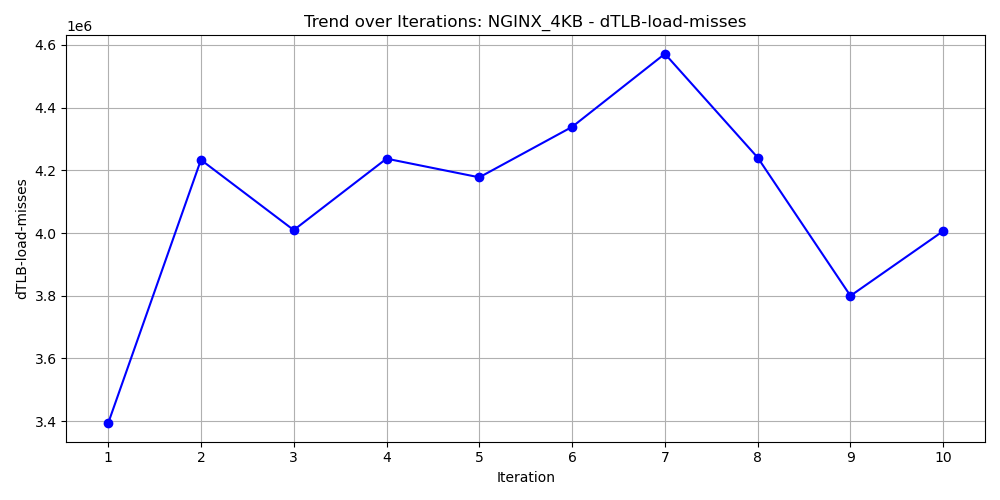
\includegraphics[width=\linewidth]{results/iterations/nginx_4kb_dtlb_trend.png}}
\caption{Nginx 4KB dTLB miss trend across 10 iterations, showing +18.1\% degradation.}
\label{fig:nginx_trend}
\end{figure}

\begin{figure}[htbp]
\centerline{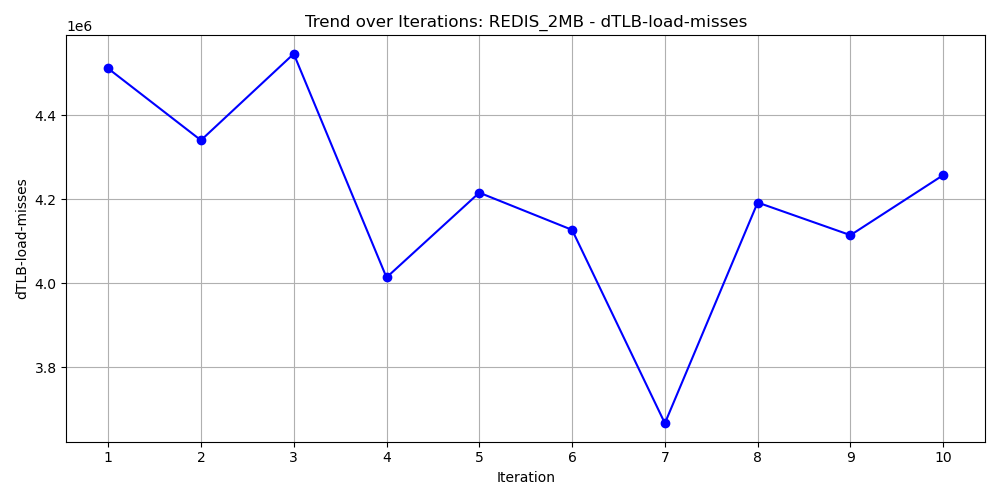
\includegraphics[width=\linewidth]{results/iterations/redis_dtlb_trend.png}}
\caption{Redis 2MB dTLB miss trend across 10 iterations.}
\label{fig:redis_trend}
\end{figure}

\begin{figure}[htbp]
\centerline{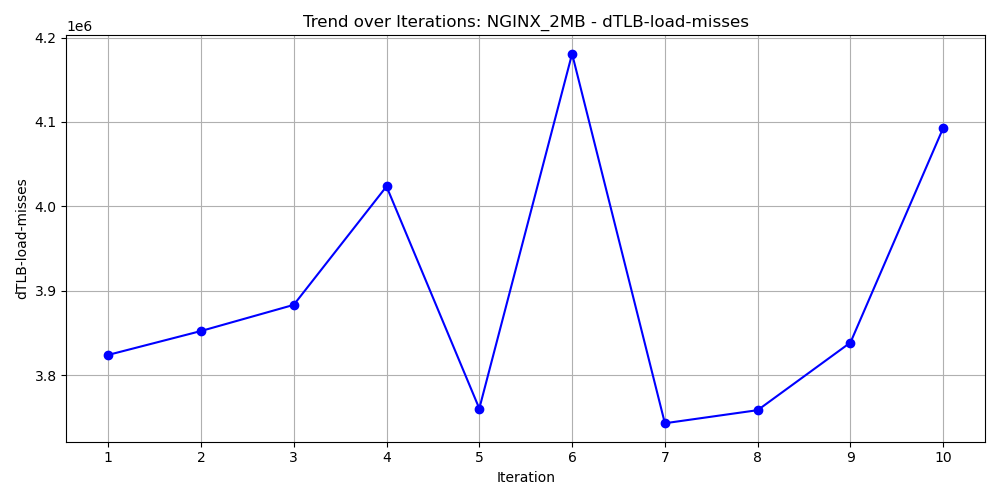
\includegraphics[width=\linewidth]{results/iterations/nginx_2mb_dtlb_trend.png}}
\caption{Nginx 2MB dTLB miss trend across 10 iterations, showing +7.0\% degradation even with THP enabled.}
\label{fig:nginx_2mb_trend}
\end{figure}

Tracking dTLB misses from iteration 1 to 10 revealed clear fragmentation patterns:
\begin{itemize}
    \item C++ 4KB: $+59.7\%$ degradation ($334{,}605 \to 534{,}379$) --- CRITICAL
    \item Nginx 4KB: $+18.1\%$ degradation ($3{,}393{,}217 \to 4{,}006{,}494$) --- CRITICAL
    \item Redis 4KB: $+11.3\%$ degradation --- CRITICAL
    \item C++ 2MB: $-8.9\%$ (stable, slight improvement)
    \item Redis 2MB: $-5.6\%$ (stable)
    \item Nginx 2MB: $+7.0\%$ (fragmentation still accumulates even with THP)
\end{itemize}
These trends empirically confirm that 4KB configurations accumulate memory fragmentation over time, while 2MB HugePage configurations remain significantly more stable across sustained operation. Even the Nginx 2MB configuration, however, is not immune: a $+7\%$ degradation over just 10 iterations highlights that \texttt{khugepaged} compaction cannot fully prevent fragmentation under sustained load.

\section{Discussion: Trade-offs and Tail Latencies}
While HugePages improve throughput for random-access workloads, they also introduce complications that can be significant in production environments.

\subsection{Memory Fragmentation}
As a system runs for extended periods, physical memory becomes fragmented with small non-contiguous allocations. When \texttt{khugepaged} attempts to collapse pages into a 2MB HugePage, it requires 512 contiguous 4KB blocks in physical memory. If the system is sufficiently fragmented, the kernel must run memory compaction routines to clear a contiguous region, which involves moving pages across physical memory locations.

\subsection{Tail Latency Spikes}
The compaction process competes with normal execution and can cause brief stalls in application threads. For latency-sensitive systems such as real-time financial applications or live streaming pipelines, these stalls appear as tail latency spikes where individual requests take substantially longer than the median. In such cases, enabling THP indiscriminately may do more harm than good, and operators should consider using explicit \texttt{hugetlbfs} reservations instead, which avoid runtime compaction entirely.

\section{Future Work}
A natural extension of this work is to evaluate 1GB pages, which are supported by modern enterprise databases such as PostgreSQL and Oracle DB. Reducing the page walk to two levels would further shrink per-miss overhead, though 1GB pages require boot-time reservation and cannot be managed transparently by \texttt{khugepaged}.

Additionally, replacing \texttt{perf} with eBPF-based tracing would allow us to instrument individual \texttt{page\_fault} kernel events and construct per-request latency histograms. This would give finer-grained visibility into translation behavior without relying on aggregate PMU averages.

\section{Conclusion}
Our 60-run multi-iteration measurement campaign confirms that page size has a workload-dependent and statistically validated impact on system performance. The synthetic benchmark demonstrates the theoretical ceiling of the benefit: enabling 2MB HugePages reduced page fault count by 99.7\% (from $131{,}463 \pm 1.26$ to $390 \pm 0.79$) and cut execution time from 0.2302s to 0.0542s. For Redis, HugePages delivered consistent throughput improvements with near-identical IPC (0.6648 vs 0.6637), confirming the gain is TLB-coverage-driven rather than cycle-efficiency-driven.

For Nginx, the raw throughput difference was negligible ($-$1.3\%), but the 2MB configuration produced \textbf{3.7$\times$ lower standard deviation} in requests-per-second, demonstrating that HugePages improve stability even for sequential workloads.

Fragmentation analysis across 10 iterations revealed that 4KB configurations degrade by up to \textbf{+59.7\%} in dTLB misses over sustained operation, while 2MB configurations remain stable or improve. The key takeaway is that HugePages are not universally beneficial in raw throughput, but they do provide systemic stability and reduce fragmentation accumulation. Engineers deploying HugePages should evaluate workload access patterns, account for background compaction tail latency, and consider explicit \texttt{hugetlbfs} reservations for latency-sensitive deployments.

\begin{thebibliography}{00}
\bibitem{b1} Linux Kernel Documentation, ``Transparent Hugepage Support,'' kernel.org, https://www.kernel.org/doc/html/latest/admin-guide/mm/transhuge.html
\bibitem{b2} Intel Corporation, ``Intel 64 and IA-32 Architectures Software Developer's Manual,'' Volume 3A: System Programming Guide, 2023.
\bibitem{b3} B. F. Cooper, A. Silberstein, E. Tam, R. Ramakrishnan, and R. Sears, ``Benchmarking Cloud Serving Systems with YCSB,'' in Proc. 1st ACM Symp. Cloud Computing (SoCC), 2010, pp. 143--154.
\bibitem{b4} Linux man-pages, ``perf-stat(1) --- Linux manual page,'' man7.org, https://man7.org/linux/man-pages/man1/perf-stat.1.html
\bibitem{b5} Nginx, Inc., ``ngx\_http\_sendfile module and kernel sendfile() optimization,'' nginx.org, 2024.
\bibitem{b6} M. Gorman, ``Understanding the Linux Virtual Memory Manager,'' Prentice Hall, 2004.
\end{thebibliography}

\end{document}